\documentclass[tikz,border=8pt]{standalone}
\usepackage{tikz}
\usetikzlibrary{arrows.meta,positioning,fit,calc}
\definecolor{ink}{HTML}{263238}
\definecolor{muted}{HTML}{60717A}
\definecolor{line}{HTML}{9AAAB2}
\definecolor{source}{HTML}{5F7180}
\definecolor{sourcefill}{HTML}{F1F4F6}
\definecolor{plan}{HTML}{2F6BBD}
\definecolor{planfill}{HTML}{EAF2FF}
\definecolor{build}{HTML}{4C8A62}
\definecolor{buildfill}{HTML}{EAF6ED}
\definecolor{check}{HTML}{C98232}
\definecolor{checkfill}{HTML}{FFF3E5}
\definecolor{publish}{HTML}{71549A}
\definecolor{publishfill}{HTML}{F3EDFF}
\tikzset{
  box/.style={rounded corners=3pt,line width=.8pt,text=ink,
    text width=3.15cm,minimum height=1.16cm,align=left,
    inner xsep=7pt,inner ysep=6pt,font=\sffamily\small},
  sourcebox/.style={box,draw=source,fill=sourcefill},
  planbox/.style={box,draw=plan,fill=planfill},
  buildbox/.style={box,draw=build,fill=buildfill},
  checkbox/.style={box,draw=check,fill=checkfill},
  publishbox/.style={box,draw=publish,fill=publishfill},
  arrow/.style={-{Latex[length=2.4mm]},line width=1pt,draw=muted},
  arrowlabel/.style={font=\sffamily\scriptsize,text=muted,fill=white,inner sep=1.5pt},
  caption/.style={font=\sffamily\scriptsize,text=muted,align=left}
}
\begin{document}
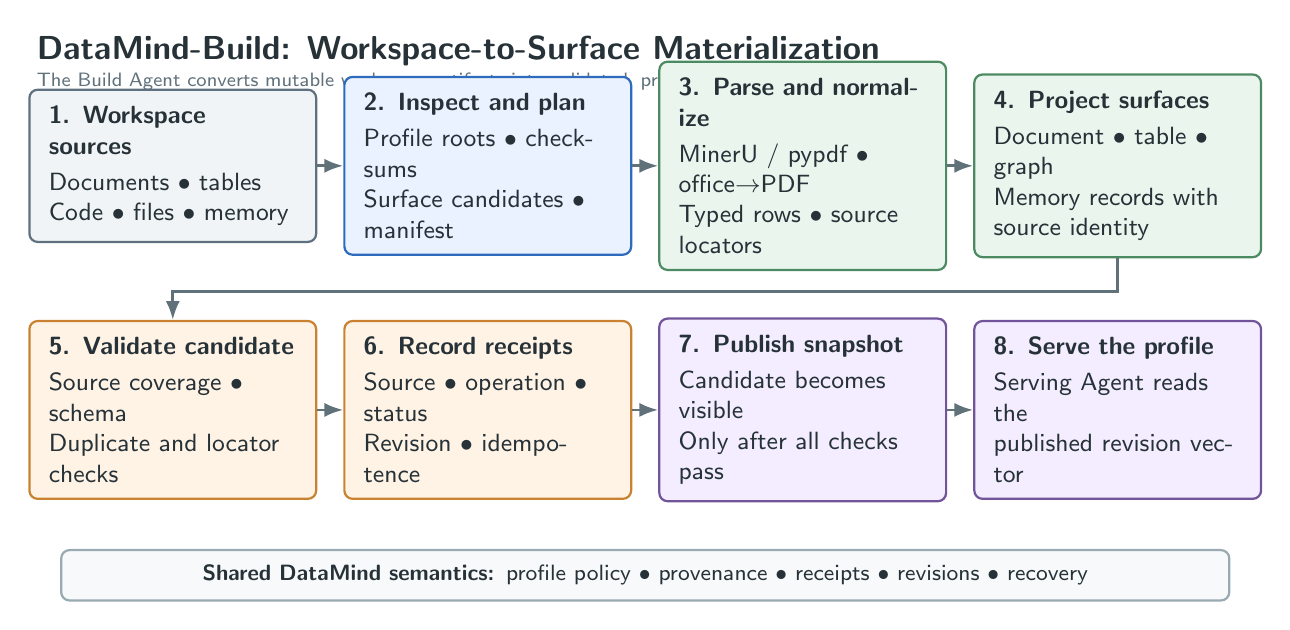
\begin{tikzpicture}[x=1cm,y=1cm]
\node[anchor=west,font=\sffamily\bfseries\large,text=ink] at (0,6.0)
  {DataMind-Build: Workspace-to-Surface Materialization};
\node[anchor=west,caption] at (0,5.62)
  {The Build Agent converts mutable workspace artifacts into validated, profile-scoped revisions.};

% Row 1: discovery and projection
\node[sourcebox] (sources) at (1.85,4.55)
  {\textbf{1. Workspace sources}\\[2pt]
   Documents $\bullet$ tables\\
   Code $\bullet$ files $\bullet$ memory};
\node[planbox] (inspect) at (5.85,4.55)
  {\textbf{2. Inspect and plan}\\[2pt]
   Profile roots $\bullet$ checksums\\
   Surface candidates $\bullet$ manifest};
\node[buildbox] (parse) at (9.85,4.55)
  {\textbf{3. Parse and normalize}\\[2pt]
   MinerU / pypdf $\bullet$ office$\to$PDF\\
   Typed rows $\bullet$ source locators};
\node[buildbox] (project) at (13.85,4.55)
  {\textbf{4. Project surfaces}\\[2pt]
   Document $\bullet$ table $\bullet$ graph\\
   Memory records with source identity};

\draw[arrow] (sources.east) -- (inspect.west);
\draw[arrow] (inspect.east) -- (parse.west);
\draw[arrow] (parse.east) -- (project.west);

% Row 2: correctness and publication
\node[checkbox] (validate) at (1.85,1.45)
  {\textbf{5. Validate candidate}\\[2pt]
   Source coverage $\bullet$ schema\\
   Duplicate and locator checks};
\node[checkbox] (receipt) at (5.85,1.45)
  {\textbf{6. Record receipts}\\[2pt]
   Source $\bullet$ operation $\bullet$ status\\
   Revision $\bullet$ idempotence};
\node[publishbox] (publish) at (9.85,1.45)
  {\textbf{7. Publish snapshot}\\[2pt]
   Candidate becomes visible\\
   Only after all checks pass};
\node[publishbox] (serve) at (13.85,1.45)
  {\textbf{8. Serve the profile}\\[2pt]
   Serving Agent reads the\\
   published revision vector};

\draw[arrow] (project.south) -- ++(0,-.42) -| (validate.north);
\draw[arrow] (validate.east) -- (receipt.west);
\draw[arrow] (receipt.east) -- (publish.west);
\draw[arrow] (publish.east) -- (serve.west);

% Shared semantics and failure boundary
\node[draw=line,fill=sourcefill!55,rounded corners=3pt,line width=.8pt,
  text width=14.6cm,minimum height=.64cm,align=center,
  font=\sffamily\footnotesize,text=ink] at (7.85,-.65)
  {\textbf{Shared DataMind semantics:} profile policy $\bullet$ provenance $\bullet$ receipts $\bullet$ revisions $\bullet$ recovery};

\end{tikzpicture}
\end{document}
